\subsection{Progettazione di dettaglio e codifica}
Periodo: dal \textbf{2022-02-14} al \textbf{2022-05-15} \mbox{} \\ \mbox{} \\
La fase inizia alla conclusione della precedente e termina con la revisione \textit{Product Baseline.} \mbox{} \\
Le precondizioni sono:
\begin{itemize}
	\item le postcondizioni della fase precedente sono state soddisfatte;
 	\item superamento della revisione \textit{Requirements and Technology Baseline}.
\end{itemize} \mbox{} \\
Le postcondizioni sono:
\begin{itemize}
	\item aggiornamento e approvazione dei documenti prodotti precedentemente;
	\item completamento codifica e verifica;
	\item stesura dell'\textit{Allegato Tecnico};
	\item redazione del \textit{Manuale Utente};
 	\item redazione del \textit{Manuale Sviluppatore};
    \item completamento della Codifica e relativa verifica del prodotto software;
    \item implementazione di tutti i requisiti obbligatori;
	\item realizzazione della presentazione da esporre nella seconda revisione: la \textit{Product Baseline}\glo{}. 
\end{itemize} \mbox{} \\
La fase è stata suddivisa in otto incrementi di sviluppo.

\pagebreak

\subsubsection{I Incremento}
\subsubsubsection{Obiettivi}
Gli obiettivi che il gruppo si prepone per questo incremento sono:
\begin{itemize}
	\item incremento e verifica della documentazione;
	\item preparazione per la progettazione e codifica.
\end{itemize}
\subsubsubsection{Periodo}
Il gruppo ritiene che il raggiungimento degli obbiettivi richiederà sette giorni di lavoro, dal \textbf{2022-02-14} al \textbf{2022-02-20}.
\subsubsubsection{Ruoli attivi}
Per raggiungere gli obiettivi il gruppo ritiene che è necessario il lavoro delle seguenti figure:
\begin{itemize}
	\item \RE{};
 	\item \AM{};
  	\item \AN{};
   	\item \PR{};
   	\item \PT{};
   	\item \VE{}.
\end{itemize}
\subsubsubsection{Attività}
Per raggiungere gli obiettivi preposti, il gruppo ritiene che dovranno essere svolte le seguenti attività:
\begin{itemize}
	\item \textbf{analisi delle tecnologie:} studio e consolidamento delle tecnologie utilizzate nel \PoC{};
 	\item \textbf{verifica:} rilevazione metriche di qualità di prodotto e di processo;
	 \item \textbf{documentazione:} 
	 \begin{itemize}
		 \item correzioni alla documentazione in base alle segnalazioni ricevute in sede di \RTB{};
		   \item riorganizzazione della pianificazione adottando gli incrementi come
		   unità base;
		  \item correzioni alla classificazione dei rischi;
		   \item calcolo del consuntivo di periodo;
		  \item calcolo del preventivo a finire rispetto alla fase;
			\item calcolo del preventivo a finire rispetto al completamento del progetto;  
		   \item inserimento nuovi termini nel \G{}.
	 \end{itemize}
\end{itemize}
\subsubsubsection{Diagramma di Gantt}
\begin{figure}[H]
	\centering
	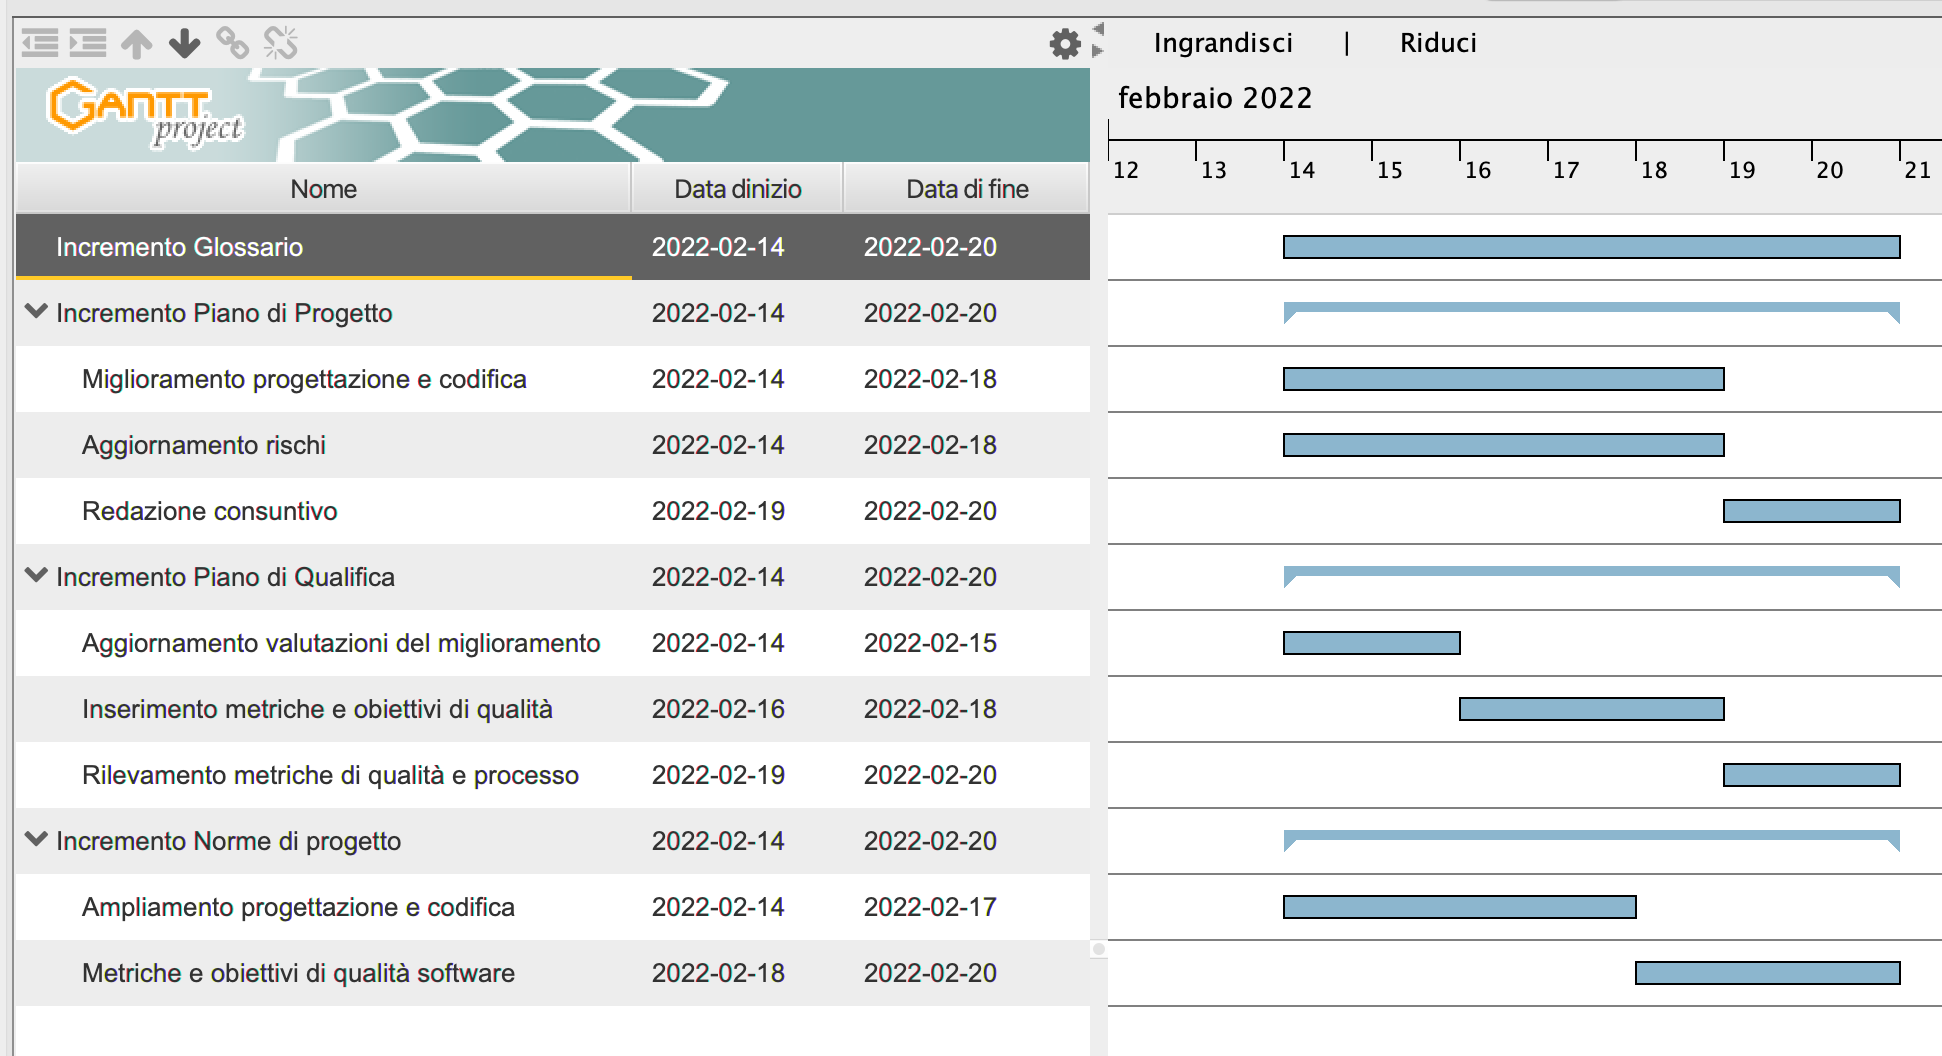
\includegraphics[scale=0.45]{Sezioni/gantt/I_incremento.png}
	\caption{Diagramma di Gantt - I Incremento, Progettazione e Codifica}
\end{figure}

\pagebreak

\subsubsection{II Incremento}
\subsubsubsection{Obiettivi}
Gli obiettivi che il gruppo si prepone per questo incremento sono:
\begin{itemize}
	\item stesura dell'\AT{} da correlare al prodotto software;
	\item preparazione per la codifica;
 \item incremento della documentazione per verifica e miglioramento continuo.
\end{itemize}
\subsubsubsection{Periodo}
Il gruppo ritiene che il raggiungimento degli obbiettivi richiederà due settimane di lavoro, dal \textbf{2022-02-21} al \textbf{2022-03-06}.
\subsubsubsection{Ruoli attivi}
Per raggiungere gli obiettivi il gruppo ritiene che è necessario il lavoro delle seguenti figure:
\begin{itemize}
	\item \RE{};
 	\item \AM{};
   	\item \PT{};
   	\item \VE{}.
\end{itemize}
\subsubsubsection{Attività}
Per raggiungere gli obiettivi preposti, il gruppo ritiene che dovranno essere svolte le seguenti attività:
\begin{itemize}
	\item \textbf{progettazione di dettaglio:} stesura dell’Allegato Tecnico: individuazione dei design pattern e creazione dei diagrammi delle classi;
 	\item \textbf{verifica:} rilevazione metriche di qualità di prodotto e di processo;
	\item \textbf{documentazione:} 
	 \begin{itemize}
		 \item correzione dell’\AdR{} a seguito dell’attività di analisi;
		   \item registrazione dell’andamento degli obiettivi di qualità;
		   \item calcolo del consuntivo di periodo;
		  \item aggiornamento delle valutazioni per il miglioramento; 
		  \item calcolo del preventivo a finire rispetto alla fase;
    	 \item inserimento nuovi termini nel \G{};
			\item calcolo del preventivo a finire rispetto al completamento del progetto.
	 \end{itemize}
\end{itemize}
\subsubsubsection{Diagramma di Gantt}
\begin{figure}[H]
	\centering
	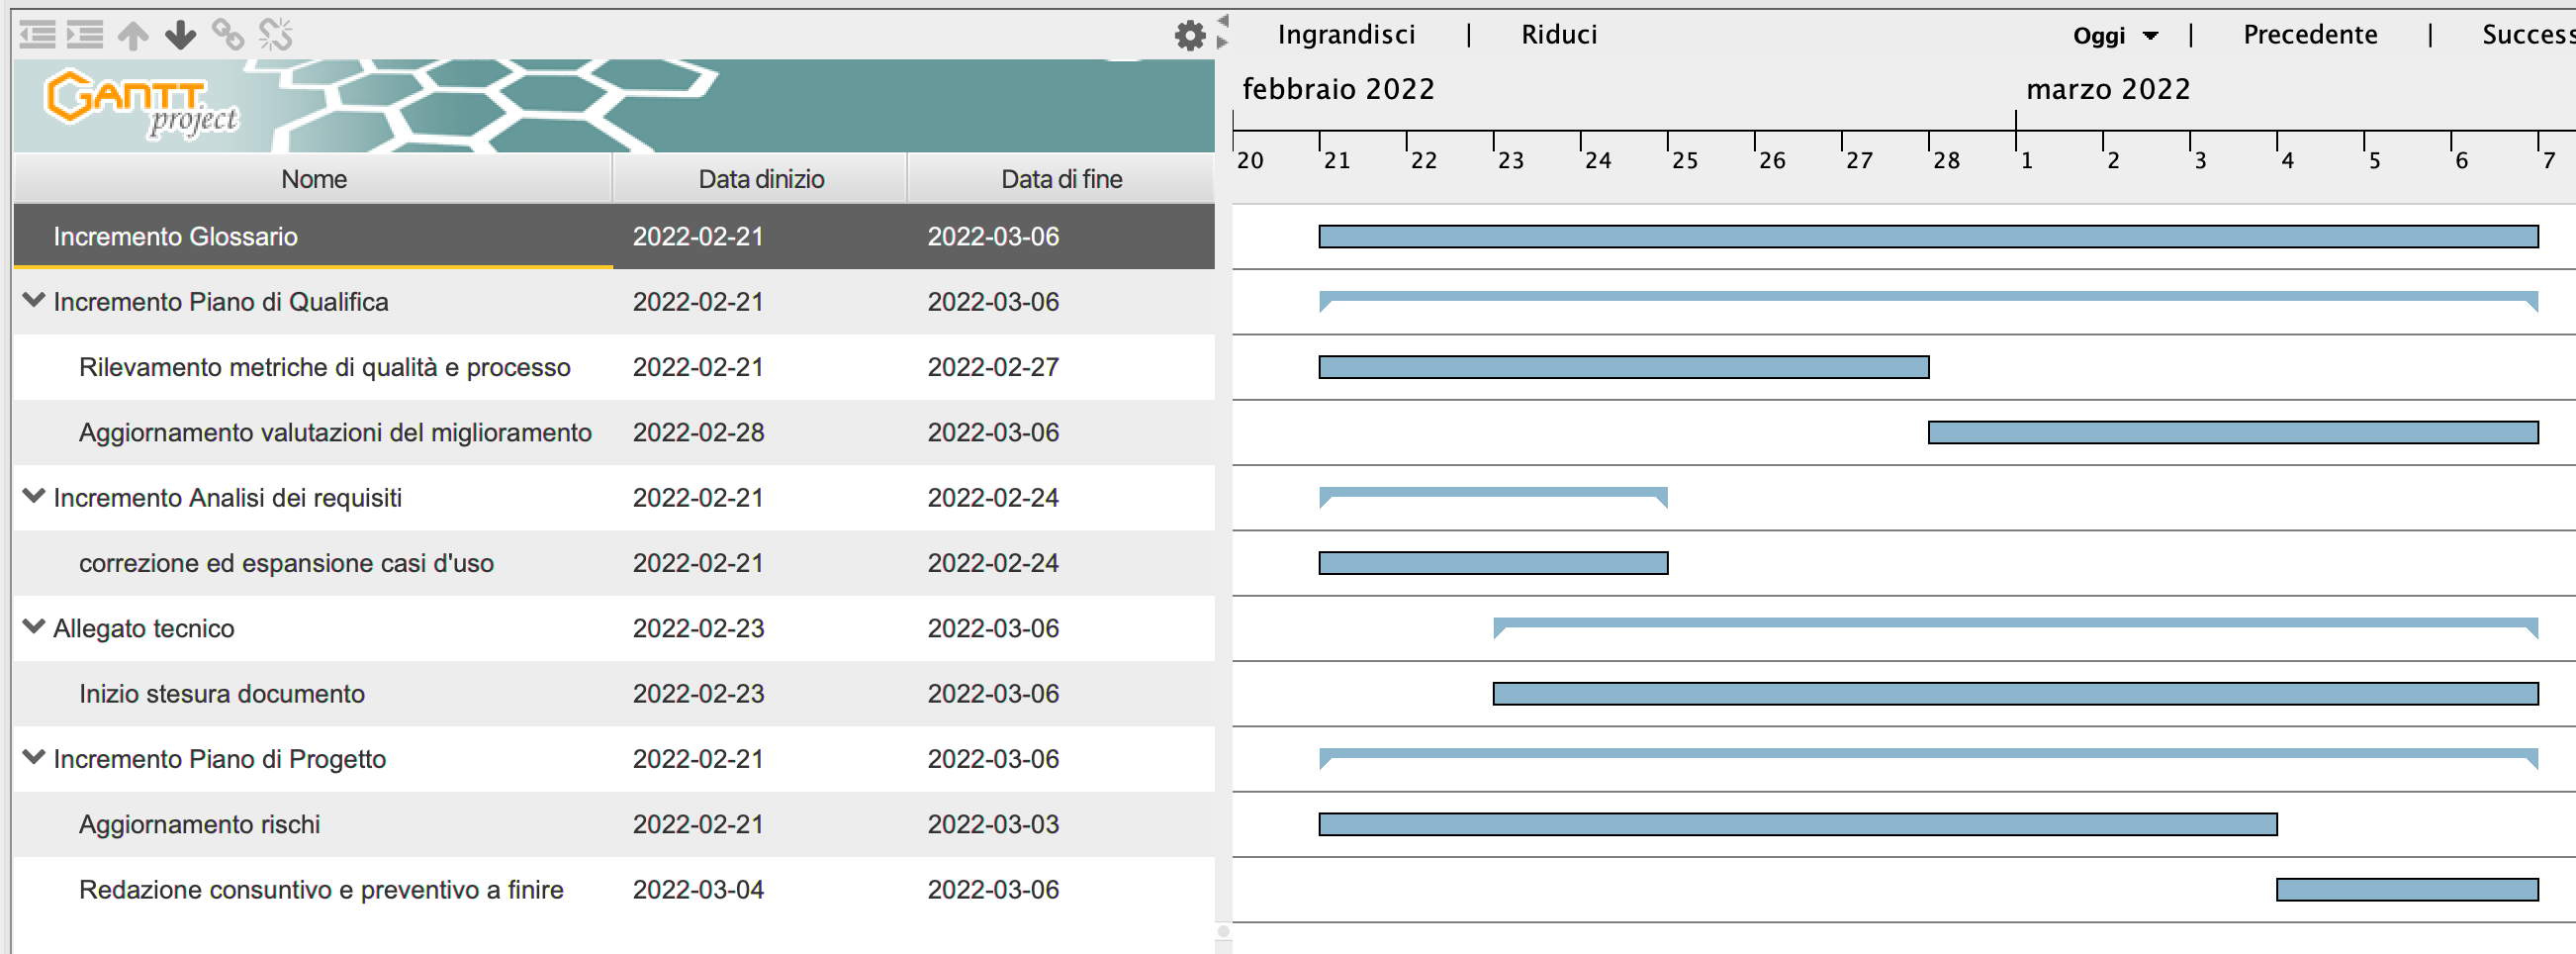
\includegraphics[scale=0.35]{Sezioni/gantt/II_incremento.png}
	\caption{Diagramma di Gantt - II Incremento, Progettazione e Codifica}
\end{figure}

\pagebreak

\subsubsection{III Incremento}
\subsubsubsection{Obiettivi}
Gli obiettivi che il gruppo si prepone per questo incremento sono:
\begin{itemize}
	\item inizio della codifica dei casi d'uso relativi alla classifica dei locali;
 	\item incremento della documentazione da correlare al prodotto software;
	\item incremento della documentazione per verifica e miglioramento continuo.
\end{itemize}
\subsubsubsection{Periodo}
Il gruppo ritiene che il raggiungimento degli obbiettivi richiederà due settimane di lavoro, dal \textbf{2022-03-07} al \textbf{2022-03-20}.
\subsubsubsection{Ruoli attivi}
Per raggiungere gli obiettivi il gruppo ritiene che è necessario il lavoro delle seguenti figure:
\begin{itemize}
	\item \RE{};
 	\item \AM{};
   	\item \PT{};
    \item \PR{};
   	\item \VE{}.
\end{itemize}
\subsubsubsection{Attività}
Per raggiungere gli obiettivi preposti, il gruppo ritiene che dovranno essere svolte le seguenti attività:
\begin{itemize}
	\item \textbf{codifica:} 
			\begin{itemize}
				\item implementazione UCW7 - Visualizzazione classifica; requisiti:
					\begin{itemize}
						\item R1FW7;
						\item R1FW7.1;
						\item R1FW7.2;
						\item R2FW7.3;
						\item R2FW7.4;
					\end{itemize}
			\end{itemize}
	\item \textbf{progettazione di dettaglio:} incremento dell’Allegato Tecnico: modifica diagrammi delle classi;
 	\item \textbf{verifica:} rilevazione metriche di qualità di prodotto e di processo;
	\item \textbf{documentazione:} 
	 \begin{itemize}
		\item inserimento nuovi termini nel \G{};
		\item stesura del \MU{} per le funzionalità completate;
		\item stesura del \MS{} per le funzionalità completate;
     	\item rilevazione delle metriche di qualità di prodotto e di processo;
     	\item rilevazione dell’andamento degli obiettivi di qualità;
		\item aggiornamento delle valutazioni per il miglioramento; 
		\item calcolo del preventivo a finire rispetto alla fase;
		\item calcolo del preventivo a finire rispetto al completamento del progetto.
	 \end{itemize}
\end{itemize}
\subsubsubsection{Diagramma di Gantt}
\begin{figure}[H]
	\centering
	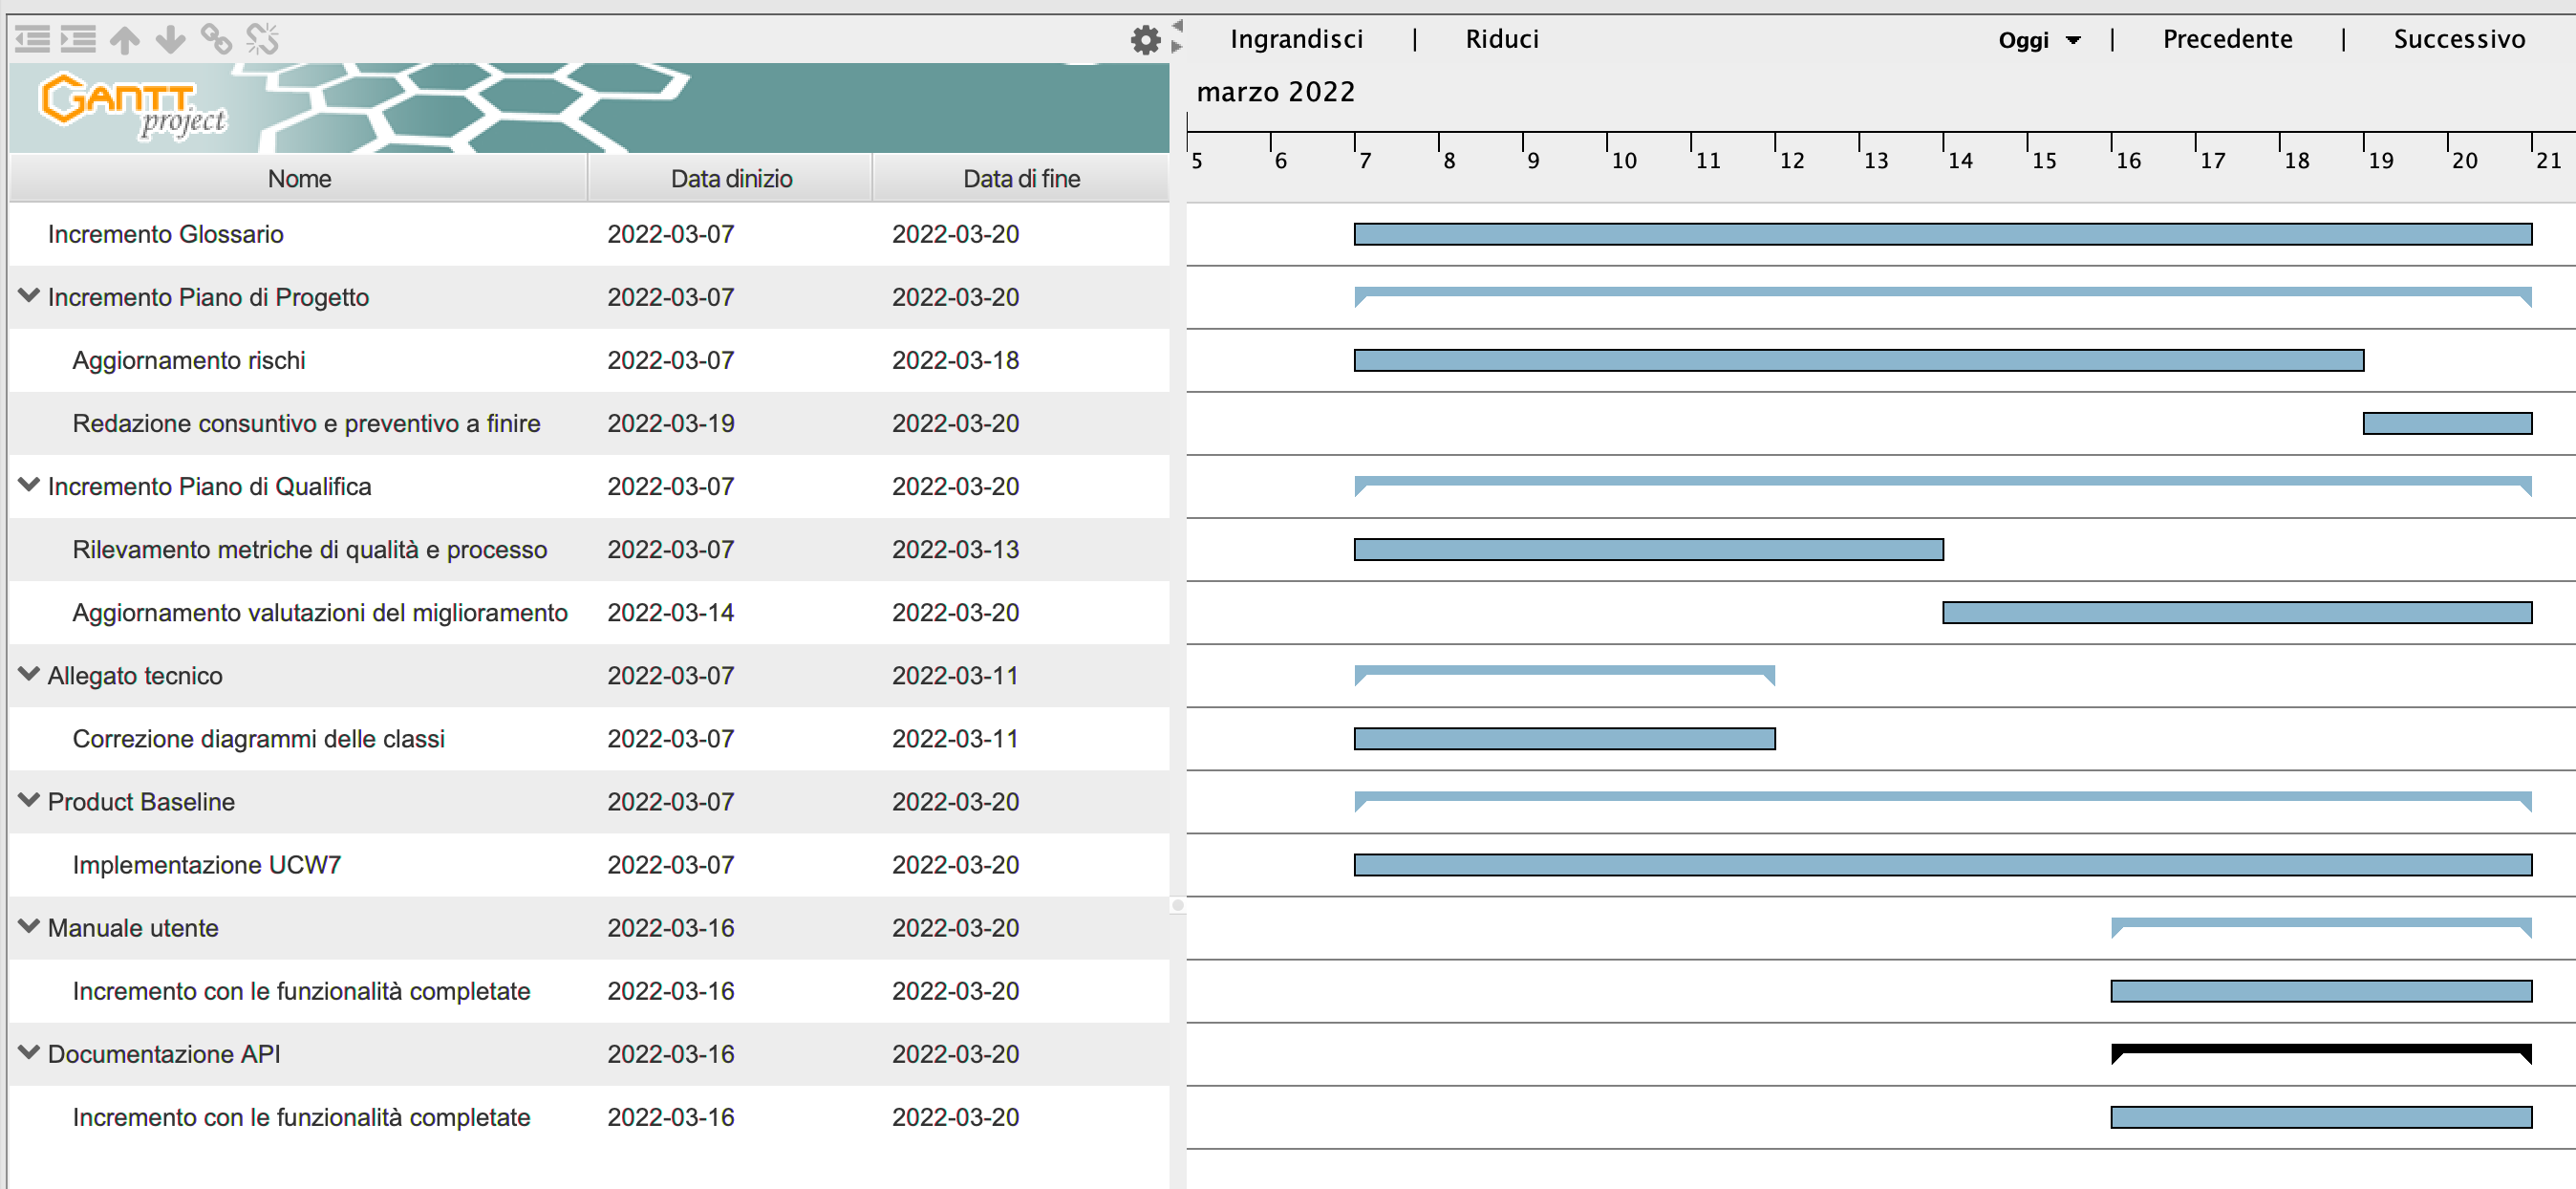
\includegraphics[scale=0.35]{Sezioni/gantt/III_incremento.png}
	\caption{Diagramma di Gantt - III Incremento, Progettazione e Codifica}
\end{figure}

\pagebreak

\subsubsection{IV Incremento}
\subsubsubsection{Obiettivi}
Gli obiettivi che il gruppo si prepone per questo incremento sono:
\begin{itemize}
	\item continuazione della codifica dei casi d'uso relativi alla classifica dei locali e alla ricerca;
 	\item incremento della documentazione da correlare al prodotto software;
	\item incremento della documentazione per verifica e miglioramento continuo.
\end{itemize}
\subsubsubsection{Periodo}
Il gruppo ritiene che il raggiungimento degli obbiettivi richiederà due settimane di lavoro, dal \textbf{2022-03-21} al \textbf{2022-04-03}.
\subsubsubsection{Ruoli attivi}
Per raggiungere gli obiettivi il gruppo ritiene che è necessario il lavoro delle seguenti figure:
\begin{itemize}
	\item \RE{};
 	\item \AM{};
   	\item \PT{};
    \item \PR{};
   	\item \VE{}.
\end{itemize}
\subsubsubsection{Attività}
Per raggiungere gli obiettivi preposti, il gruppo ritiene che dovranno essere svolte le seguenti attività:
\begin{itemize}
	\item \textbf{codifica:} 
			\begin{itemize}
				\item implementazione UCW10 - Ricerca di un locale tramite nome; requisiti:
					\begin{itemize}
						\item R1FW10;
					\end{itemize}
				\item implementazione UCW11 - Visualizza informazioni locale ; requisiti:
					\begin{itemize}
						\item R2FW11;
						\item R2FW11.1;
						\item R2FW11.2;
						\item R2FW11.3;
						\item R2FW11.4;
      					\item R1FW11.1.1;
           				\item R2FW11.1.2;
               			\item R2FW11.1.3;
                  		\item R3FW11.1.4;
                   		\item R2FW11.1.5;
						\item R2FW11.1.6;
						\item R1FW11.2.1;
						\item R1FW11.2.2;
						\item R1FW11.2.3;
						\item R1FW11.2.4;
						\item R2FW11.3.1;
						\item R2FW11.3.2;
						\item R2FW11.3.3;
					\end{itemize}
				\item implementazione UCW12 - Inserimento locale nella lista dei preferiti; requisiti:
					\begin{itemize}
						\item R2FW12;
					\end{itemize}
				\item implementazione UCW13 - Rimozione locale dalla lista dei preferiti; requisiti:
					\begin{itemize}
						\item R2FW13;
					\end{itemize}
			\end{itemize}
	\item \textbf{progettazione di dettaglio:} incremento dell’Allegato Tecnico: aggiunta diagrammi di sequenza;
 	\item \textbf{verifica:} rilevazione metriche di qualità di prodotto e di processo;
	\item \textbf{documentazione:} 
	 \begin{itemize}
		\item inserimento nuovi termini nel \G{};
		\item stesura del \MU{} per le funzionalità completate;
		\item stesura del \MS{} per le funzionalità completate;
  		\item registrazione degli esiti della verifica;
     	\item registrazione dell’andamento degli obiettivi di qualità;
		\item aggiornamento delle valutazioni per il miglioramento; 
		\item calcolo del preventivo a finire rispetto alla fase;
		\item calcolo del preventivo a finire rispetto al completamento del progetto.
	 \end{itemize}
\end{itemize}
\subsubsubsection{Diagramma di Gantt}
\begin{figure}[H]
	\centering
	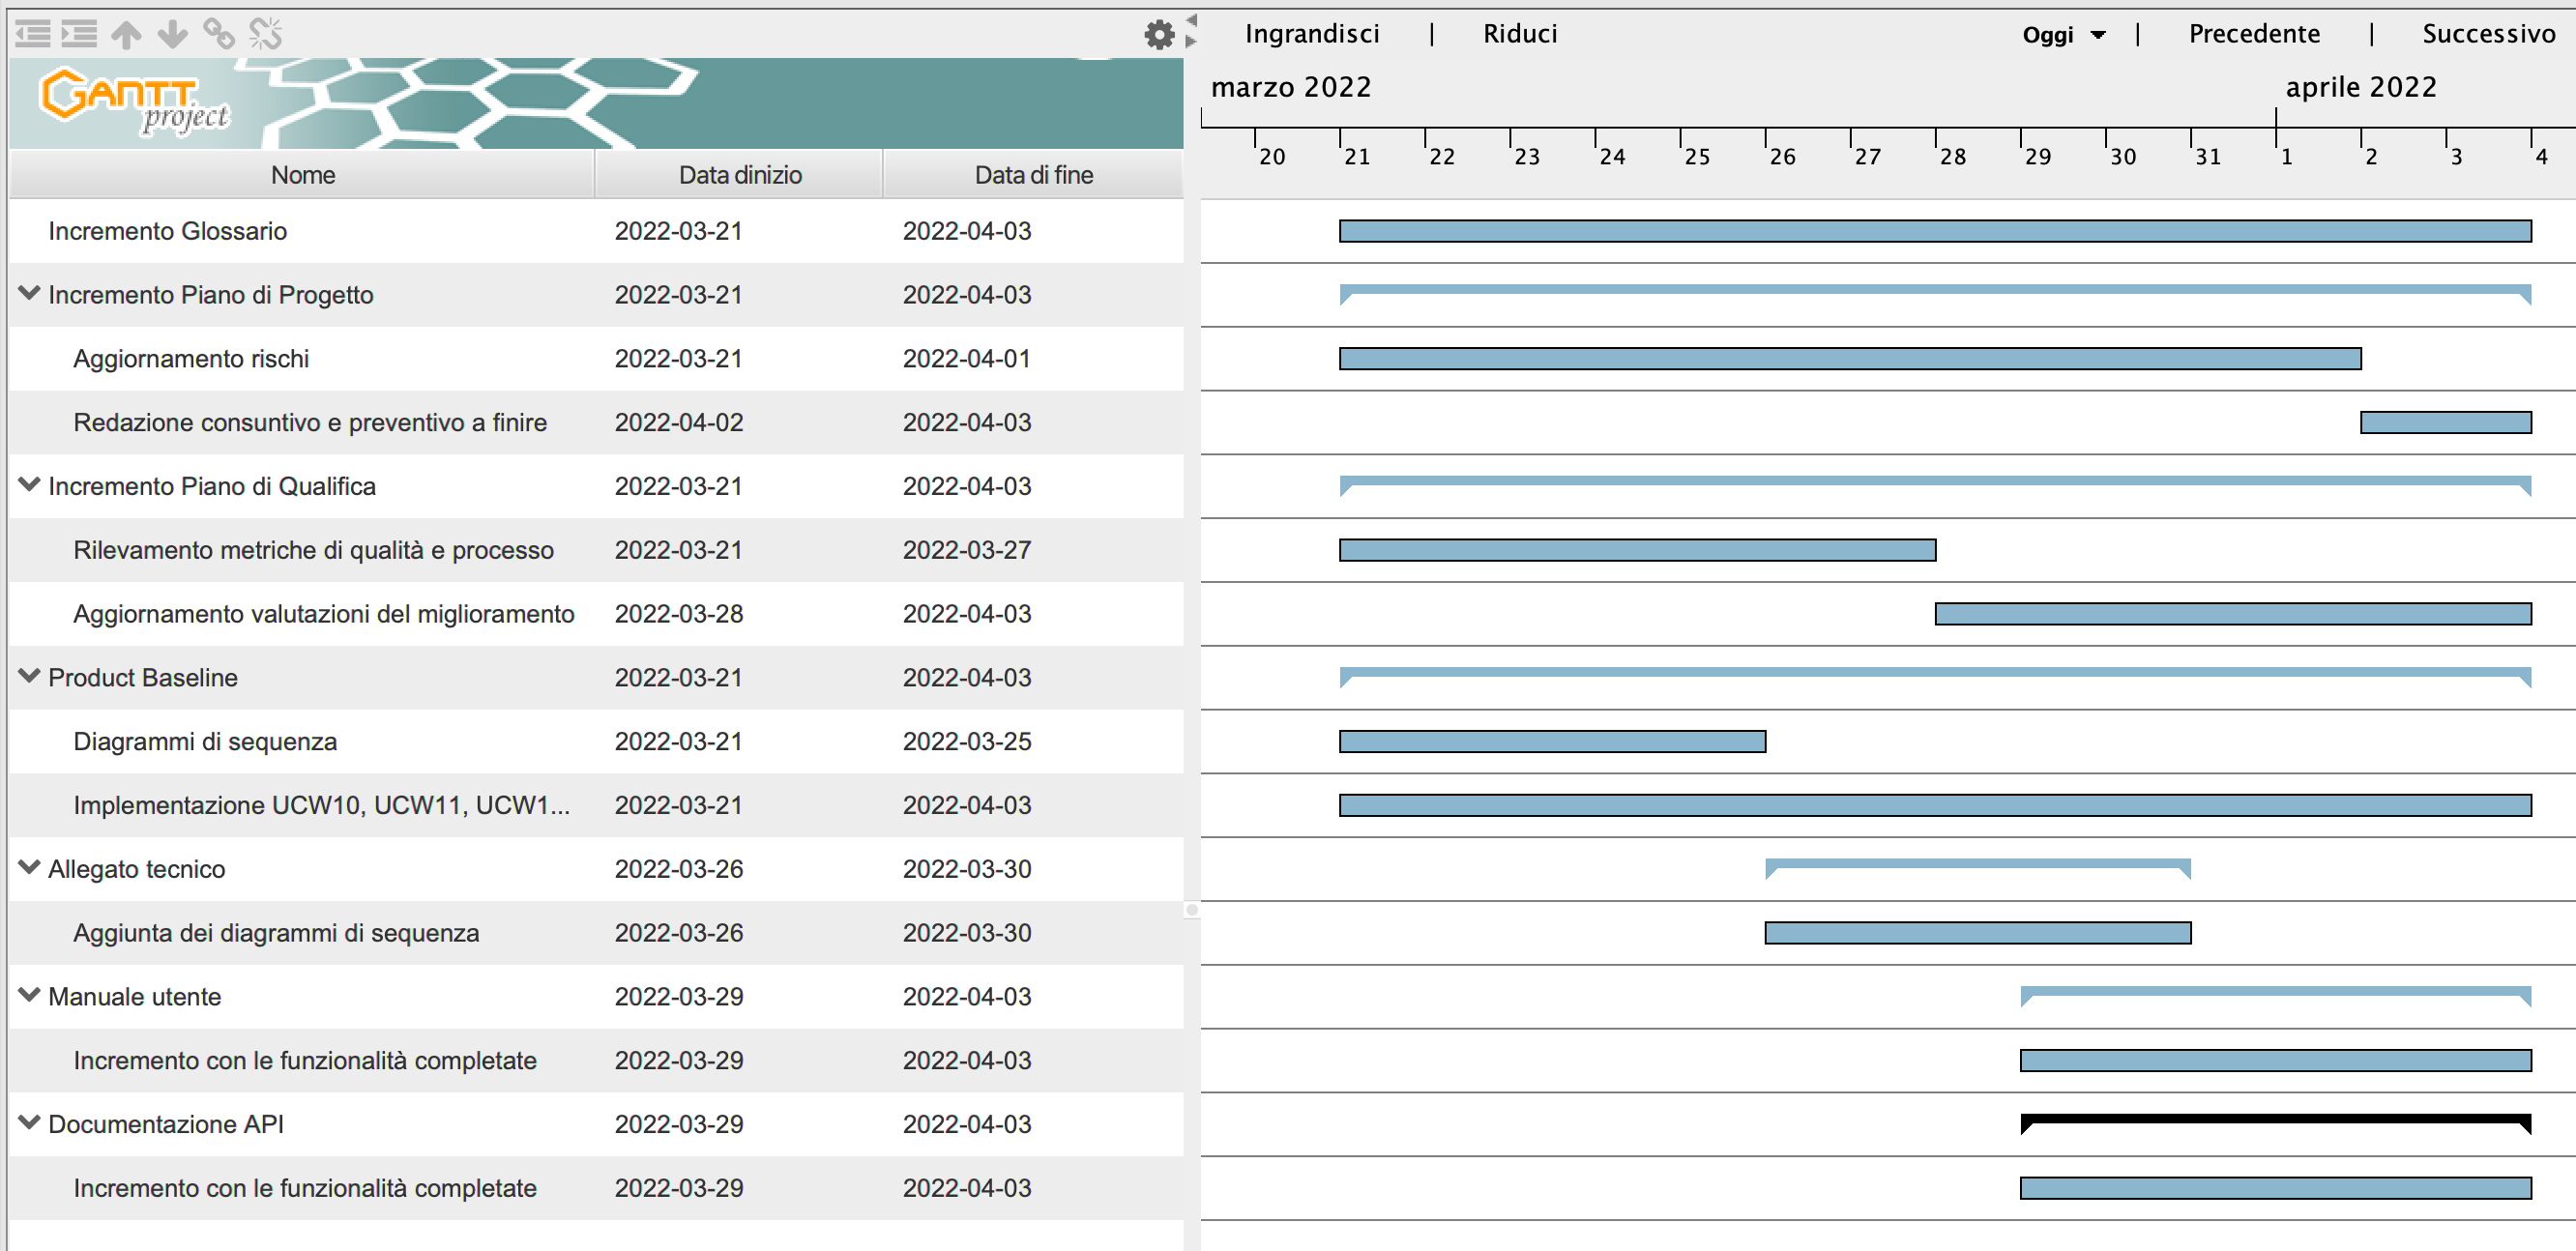
\includegraphics[scale=0.35]{Sezioni/gantt/IV_incremento.png}
	\caption{Diagramma di Gantt - IV Incremento, Progettazione e Codifica}
\end{figure}

\pagebreak

\subsubsection{V Incremento}
\subsubsubsection{Obiettivi}
Gli obiettivi che il gruppo si prepone per questo incremento sono:
\begin{itemize}
	\item inizio  della codifica dei casi d'uso relativi al login e all'area personale;
 	\item incremento della documentazione da correlare al prodotto software;
	\item incremento della documentazione per verifica e miglioramento continuo.
\end{itemize}
\subsubsubsection{Periodo}
Il gruppo ritiene che il raggiungimento degli obbiettivi richiederà una settimana di lavoro, dal \textbf{2022-04-04} al \textbf{2022-04-10}.
\subsubsubsection{Ruoli attivi}
Per raggiungere gli obiettivi il gruppo ritiene che è necessario il lavoro delle seguenti figure:
\begin{itemize}
	\item \RE{};
 	\item \AM{};
   	\item \PT{};
    \item \PR{};
   	\item \VE{}.
\end{itemize}
\subsubsubsection{Attività}
Per raggiungere gli obiettivi preposti, il gruppo ritiene che dovranno essere svolte le seguenti attività:
\begin{itemize}
	\item \textbf{codifica:} 
			\begin{itemize}
				\item implementazione UCW1 - Registrazione; requisiti:
					\begin{itemize}
						\item R1FW1
					\end{itemize}
				\item implementazione UCW2 - Login; requisiti:
					\begin{itemize}
						\item R1FW2
					\end{itemize}
				\item implementazione UCW3 - Recupero password; requisiti:
					\begin{itemize}
						\item R1FW3
					\end{itemize}
			\end{itemize}
 	\item \textbf{verifica:} rilevazione metriche di qualità di prodotto e di processo;
	\item \textbf{documentazione:} 
	 \begin{itemize}
		\item inserimento nuovi termini nel \G{};
		\item stesura del \MU{} per le funzionalità completate;
		\item stesura del \MS{} per le funzionalità completate;
  		\item registrazione degli esiti della verifica;
     	\item registrazione dell’andamento degli obiettivi di qualità;
		\item aggiornamento delle valutazioni per il miglioramento; 
		\item calcolo del preventivo a finire rispetto alla fase;
		\item calcolo del preventivo a finire rispetto al completamento del progetto.
	 \end{itemize}
\end{itemize}
\subsubsubsection{Diagramma di Gantt}
\begin{figure}[H]
	\centering
	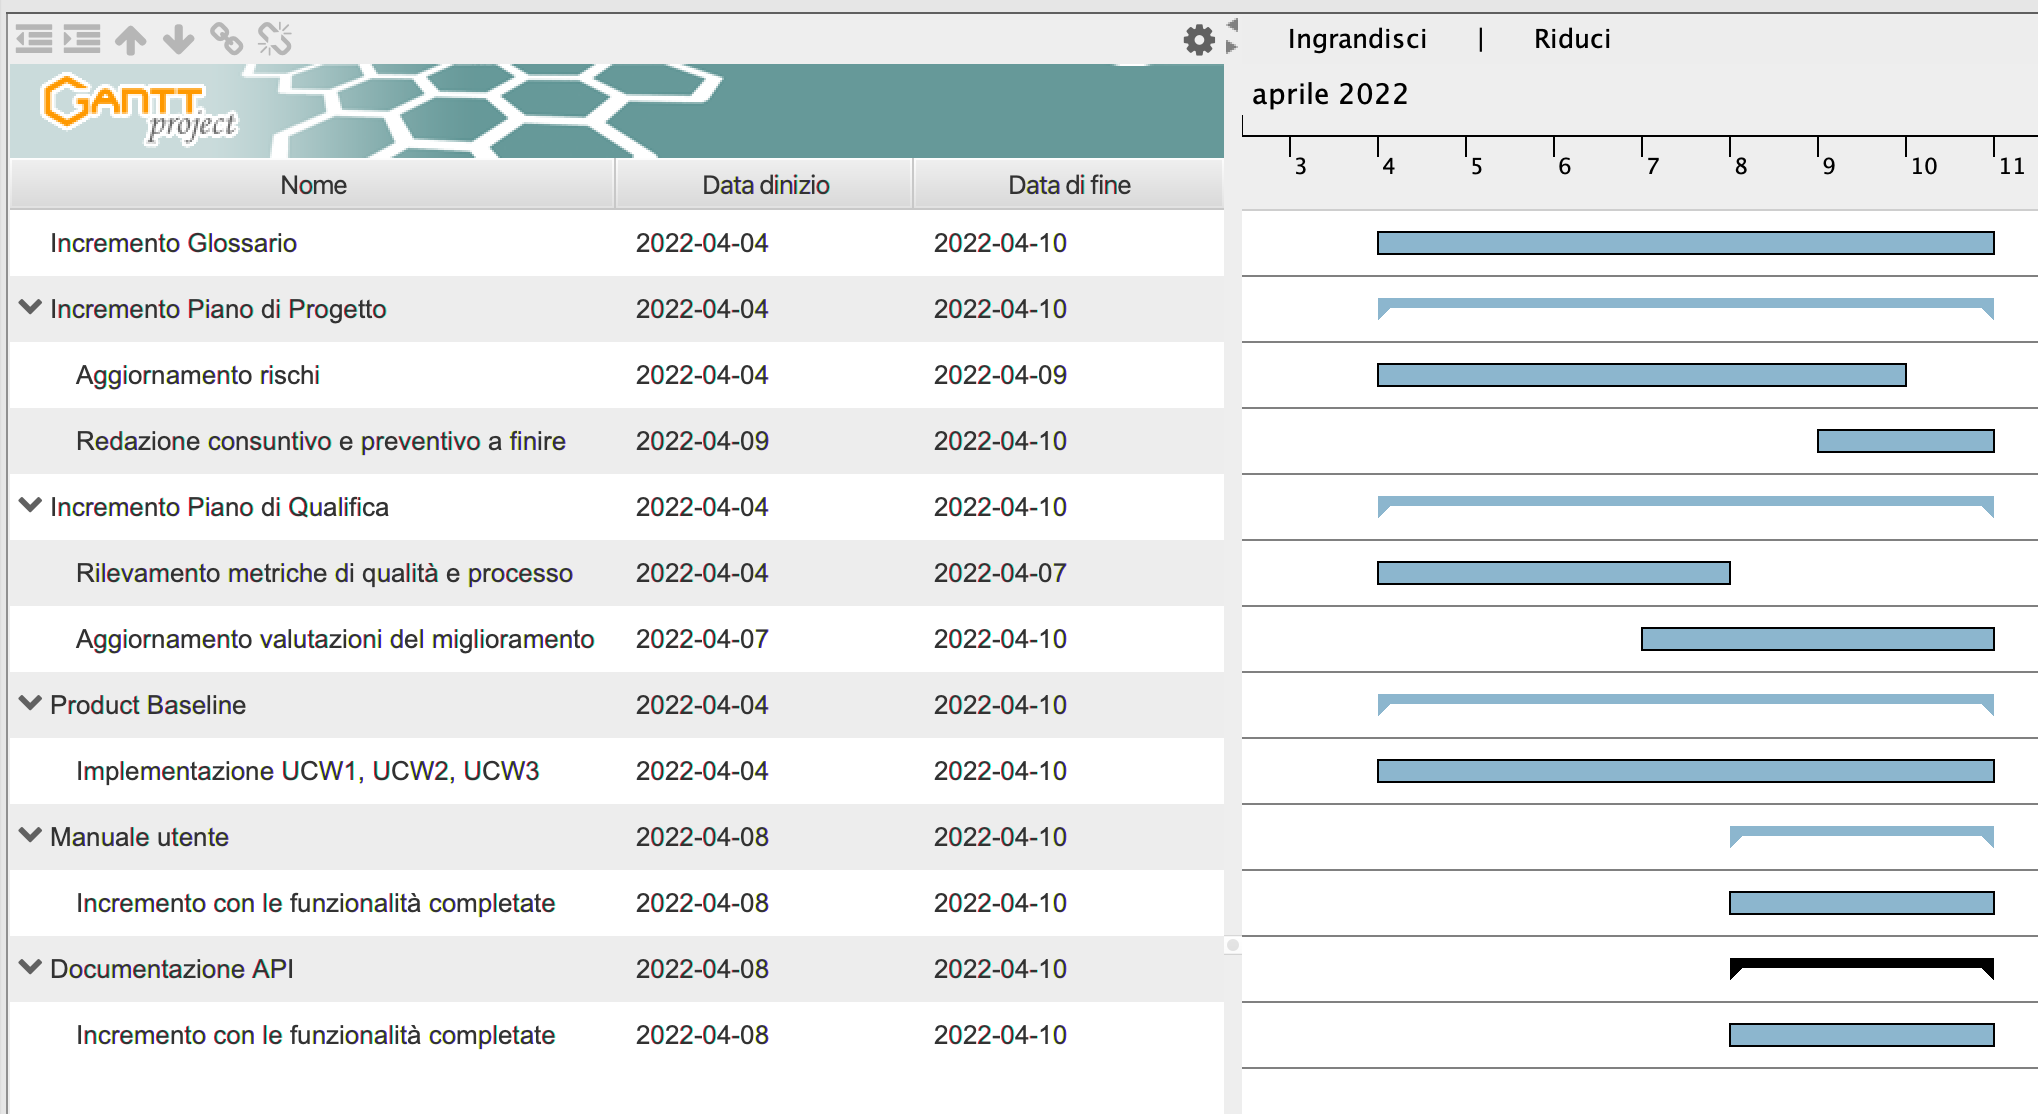
\includegraphics[scale=0.45]{Sezioni/gantt/V_incremento.png}
	\caption{Diagramma di Gantt - V Incremento, Progettazione e Codifica}
\end{figure}

\pagebreak

\subsubsection{VI Incremento}
\subsubsubsection{Obiettivi}
Gli obiettivi che il gruppo si prepone per questo incremento sono:
\begin{itemize}
	\item conclusione della codifica dei casi d'uso relativi al login e all'area personale;
 	\item incremento della documentazione da correlare al prodotto software;
	\item incremento della documentazione per verifica e miglioramento continuo.
\end{itemize}
\subsubsubsection{Periodo}
Il gruppo ritiene che il raggiungimento degli obbiettivi richiederà una settimana di lavoro, dal \textbf{2022-04-11} al \textbf{2022-04-16}.
\subsubsubsection{Ruoli attivi}
Per raggiungere gli obiettivi il gruppo ritiene che è necessario il lavoro delle seguenti figure:
\begin{itemize}
	\item \RE{};
 	\item \AM{};
   	\item \PT{};
    \item \PR{};
   	\item \VE{}.
\end{itemize}
\subsubsubsection{Attività}
Per raggiungere gli obiettivi preposti, il gruppo ritiene che dovranno essere svolte le seguenti attività:
\begin{itemize}
	\item \textbf{codifica:} 
			\begin{itemize}
				\item implementazione UCW4 - Area personale; requisiti:
					\begin{itemize}
						\item R1FW4;
      					\item R1FW4.1;
           				\item R1FW4.2;
               			\item R1FW4.3
					\end{itemize}
				\item implementazione UCW5 - Proposta profilo Instagram; requisiti:
					\begin{itemize}
						\item R1FW5;
					\end{itemize}
			\end{itemize}
 	\item \textbf{verifica:} rilevazione metriche di qualità di prodotto e di processo;
	\item \textbf{documentazione:} 
	 \begin{itemize}
		\item inserimento nuovi termini nel \G{};
		\item completamento del \MU{};
		\item completamento del \MS{};
  		\item registrazione degli esiti della verifica;
     	\item registrazione dell’andamento degli obiettivi di qualità;
		\item aggiornamento delle valutazioni per il miglioramento; 
		\item calcolo del preventivo a finire rispetto alla fase;
		\item calcolo del preventivo a finire rispetto al completamento del progetto.
	 \end{itemize}
\end{itemize}
\subsubsubsection{Diagramma di Gantt}
\begin{figure}[H]
	\centering
	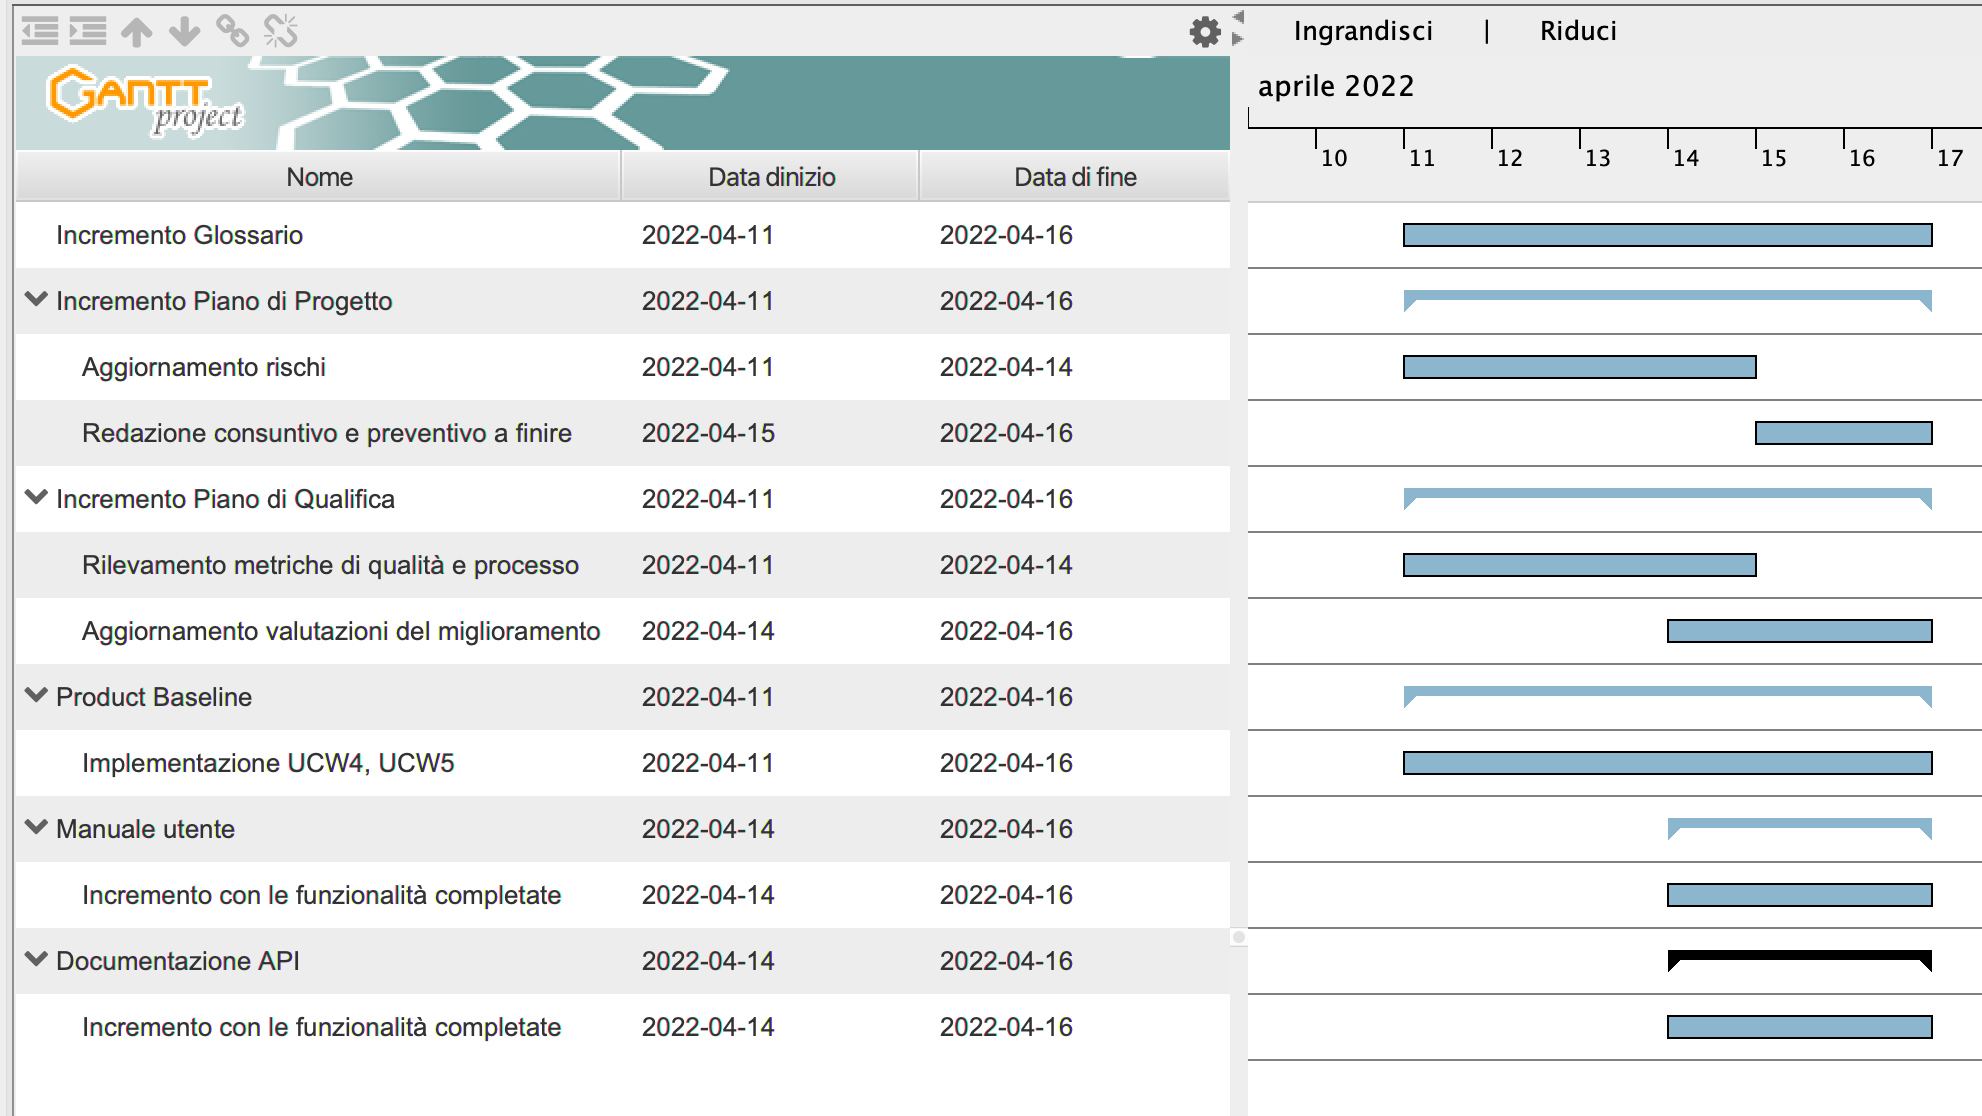
\includegraphics[scale=0.45]{Sezioni/gantt/VI_incremento.png}
	\caption{Diagramma di Gantt - VI Incremento, Progettazione e Codifica}
\end{figure}

\pagebreak

\subsubsection{VII Incremento}
\subsubsubsection{Obiettivi}
Gli obiettivi che il gruppo si prepone per questo incremento sono:
\begin{itemize}
 	\item perfezionamento del codice;
  	\item risoluzione di alcune problematiche legate al crawler;
  	\item correzione dei bug individuati da test più approfonditi;
 	\item incremento della documentazione da correlare al prodotto software;
	\item incremento della documentazione per verifica e miglioramento continuo.
\end{itemize}
\subsubsubsection{Periodo}
Il gruppo ritiene che il raggiungimento degli obbiettivi richiederà due settimane di lavoro, dal \textbf{2022-04-19} al \textbf{2022-05-08}.
\subsubsubsection{Ruoli attivi}
Per raggiungere gli obiettivi il gruppo ritiene che è necessario il lavoro delle seguenti figure:
\begin{itemize}
	\item \RE{};
 	\item \AM{};
    \item \PR{};
   	\item \VE{}.
\end{itemize}
\subsubsubsection{Attività}
Per raggiungere gli obiettivi preposti, il gruppo ritiene che dovranno essere svolte le seguenti attività:
\begin{itemize}
	\item \textbf{codifica:} 
			\begin{itemize}
				\item perfezionamento dell'attività del crawler;
				\item correzione dei bug individuati;
    			\item correzione in base alle segnalazioni ricevute in sede di colloquio con proponente.
			\end{itemize}
 	\item \textbf{verifica:} rilevazione metriche di qualità di prodotto e di processo;
	\item \textbf{documentazione:} 
	 \begin{itemize}
		\item inserimento nuovi termini nel \G{};
  		\item registrazione degli esiti della verifica;
     	\item registrazione dell’andamento degli obiettivi di qualità;
		\item aggiornamento delle valutazioni per il miglioramento; 
		\item calcolo del preventivo a finire rispetto alla fase;
		\item calcolo del preventivo a finire rispetto al completamento del progetto.
	 \end{itemize}
\end{itemize}
\subsubsubsection{Diagramma di Gantt}
\begin{figure}[H]
	\centering
	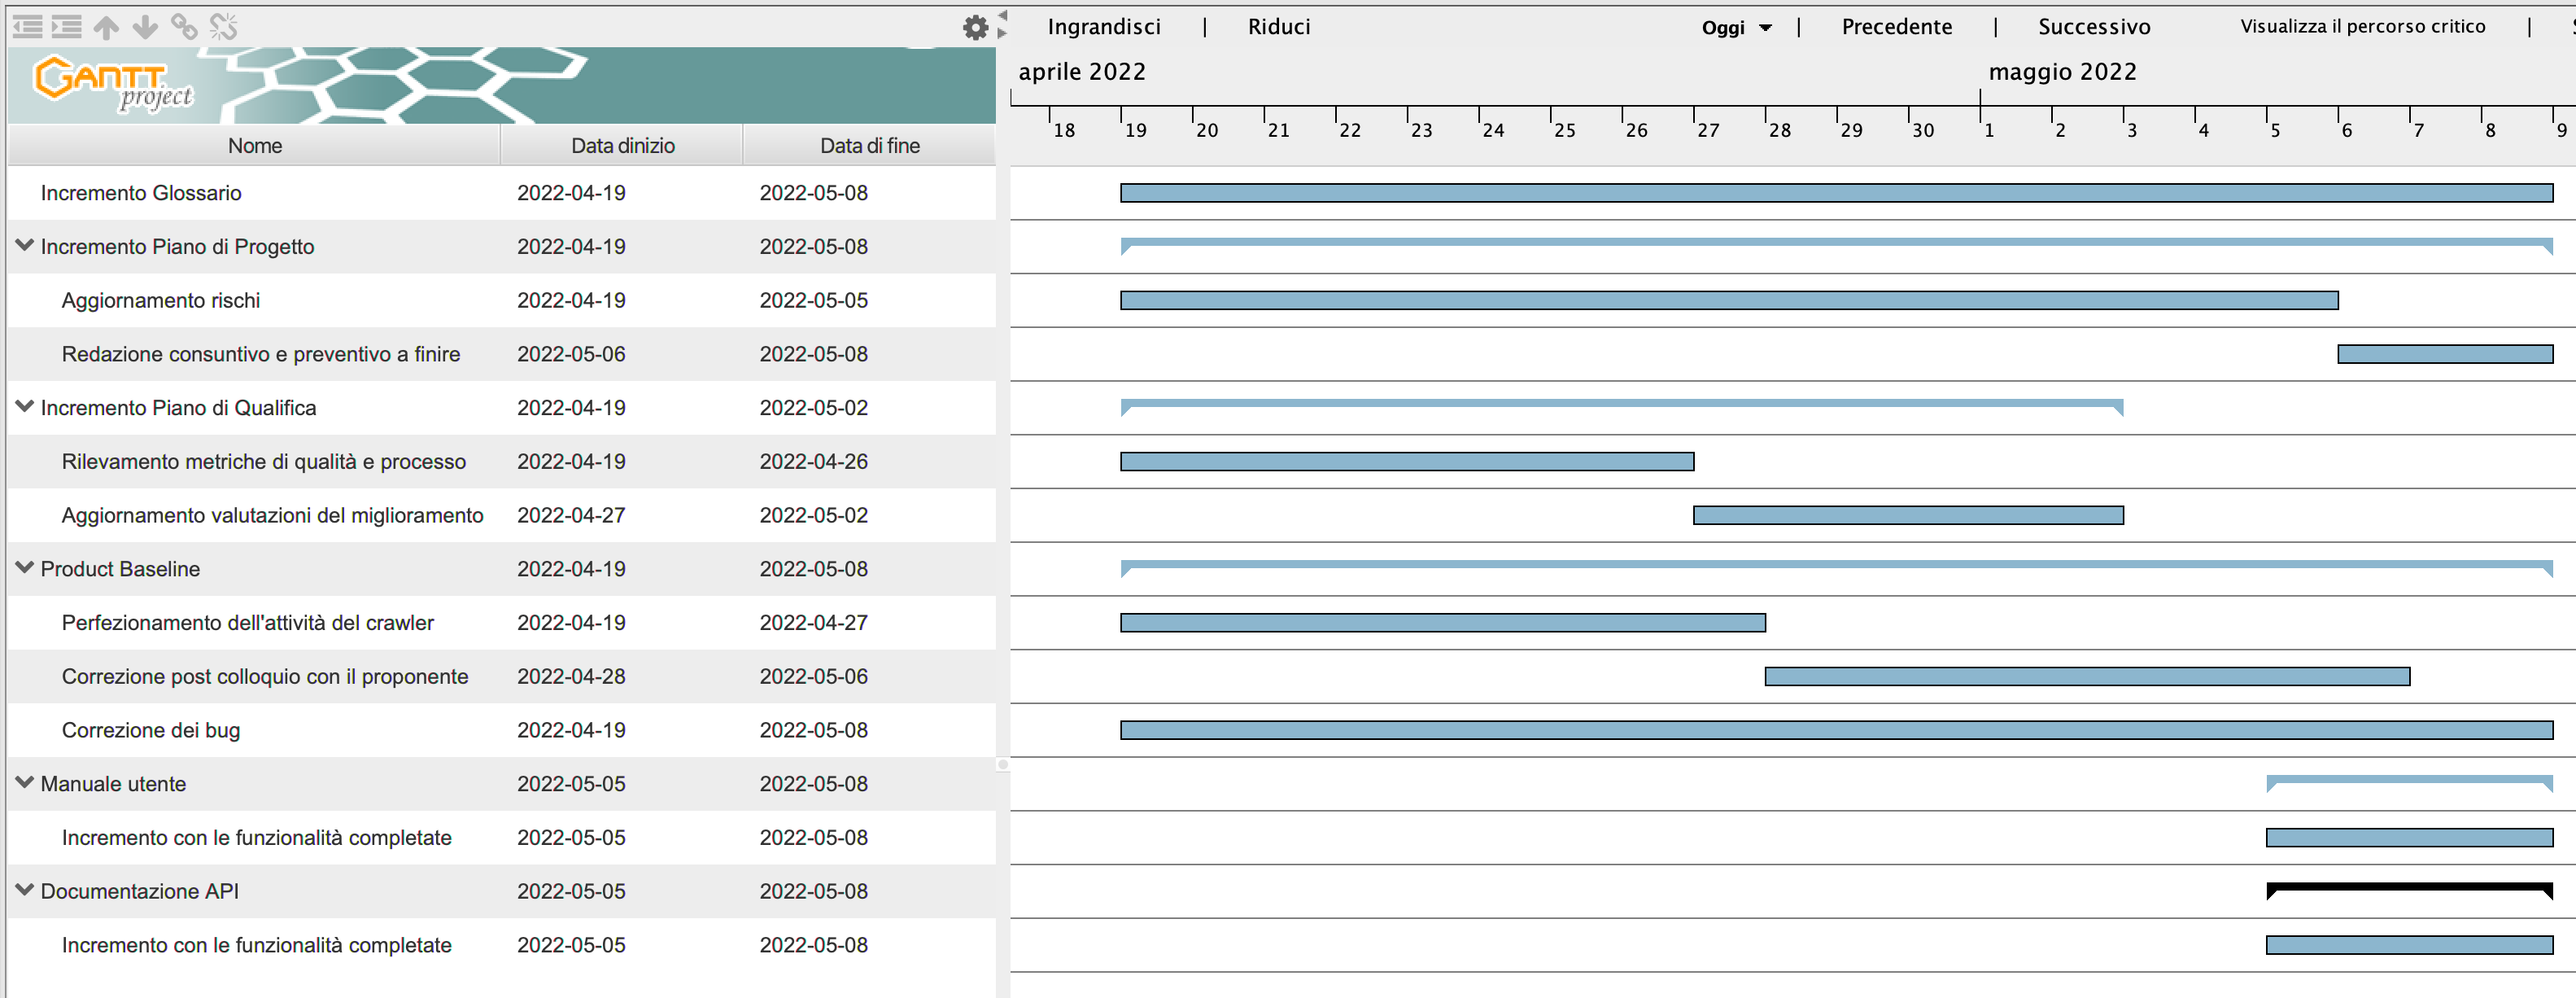
\includegraphics[scale=0.30]{Sezioni/gantt/VII_incremento.png}
	\caption{Diagramma di Gantt - VII Incremento, Progettazione e Codifica}
\end{figure}

\pagebreak

\subsubsection{VIII Incremento}
\subsubsubsection{Obiettivi}
Gli obiettivi che il gruppo si prepone per questo incremento sono:
\begin{itemize}
	\item preparazione all’esposizione della revisione \PB{};
  	\item preparazione della lettera di presentazione;
 	\item incremento della documentazione da correlare al prodotto software;
	\item incremento della documentazione per verifica e miglioramento continuo.
\end{itemize}
\subsubsubsection{Periodo}
Il gruppo ritiene che il raggiungimento degli obbiettivi richiederà una settimana di lavoro, dal \textbf{2022-05-09} al \textbf{2022-05-15}.
\subsubsubsection{Ruoli attivi}
Per raggiungere gli obiettivi il gruppo ritiene che è necessario il lavoro delle seguenti figure:
\begin{itemize}
	\item \RE{};
 	\item \AM{};
   	\item \PT{};
    \item \PR{};
   	\item \VE{}.
\end{itemize}
\subsubsubsection{Attività}
Per raggiungere gli obiettivi preposti, il gruppo ritiene che dovranno essere svolte le seguenti attività:
\begin{itemize}
 	\item \textbf{verifica:} rilevazione metriche di qualità di prodotto e di processo;
	\item \textbf{documentazione:} 
	 \begin{itemize}
		\item inserimento nuovi termini nel \G{};
  		\item registrazione degli esiti della verifica;
     	\item registrazione dell’andamento degli obiettivi di qualità;
      	\item aggiornamento della classificazione e rilevazione dei rischi;
		\item aggiornamento delle valutazioni per il miglioramento; 
		\item calcolo del preventivo a finire rispetto alla fase;
		\item calcolo del preventivo a finire rispetto al completamento del progetto.
	 \end{itemize}
\end{itemize}
\subsubsubsection{Diagramma di Gantt}
\begin{figure}[H]
	\centering
	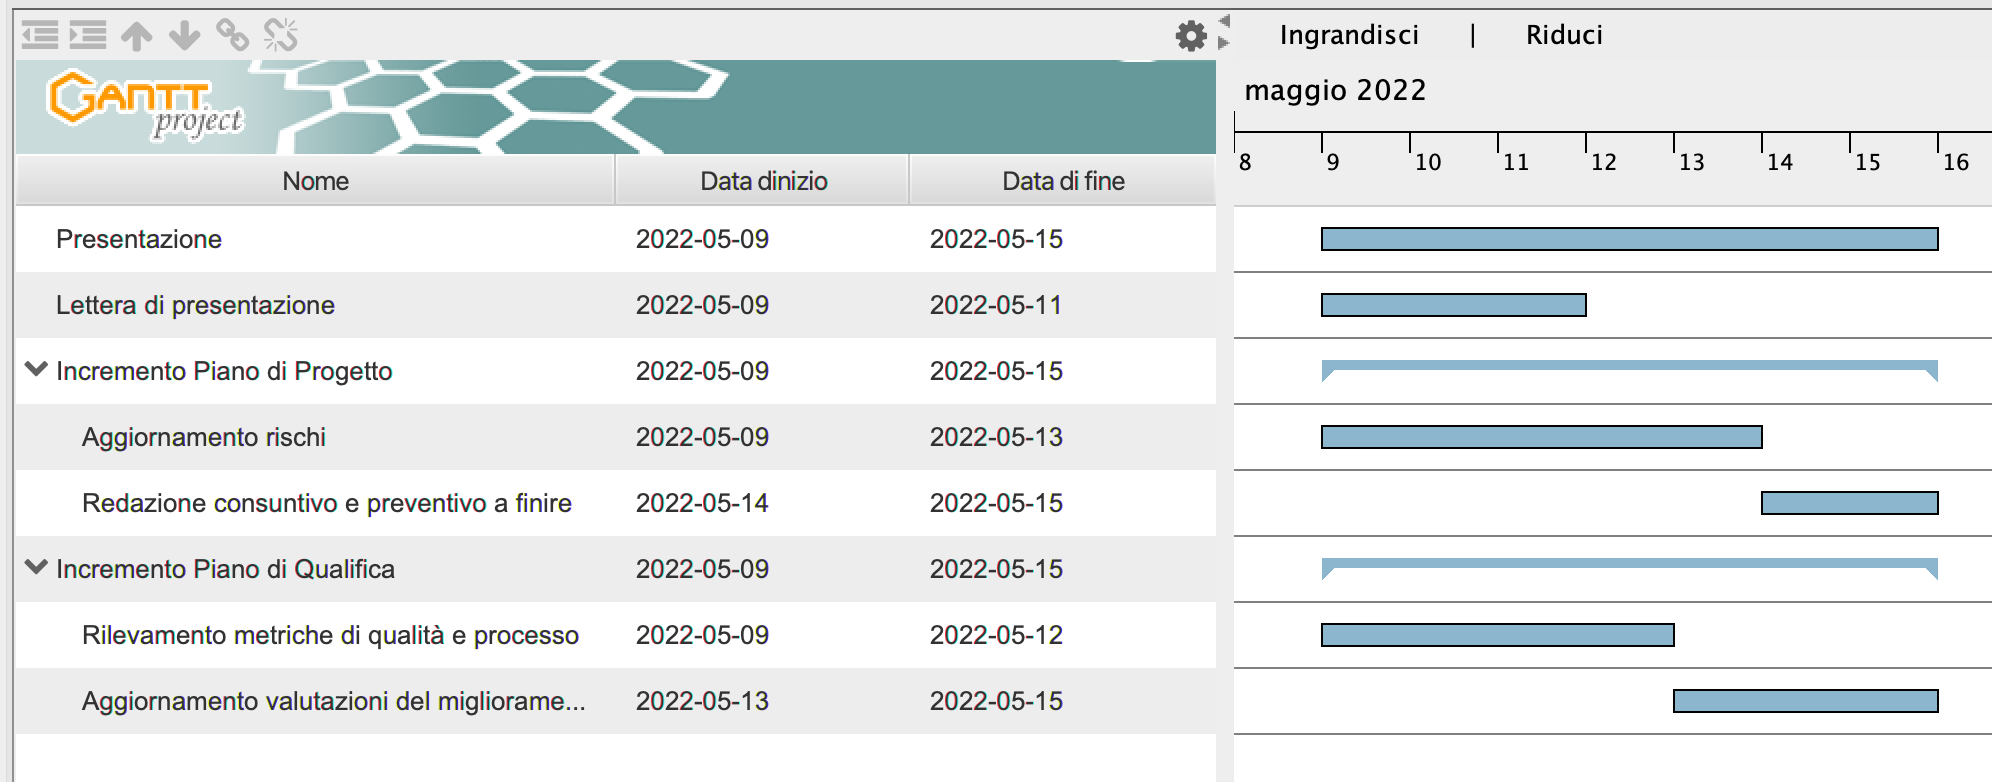
\includegraphics[scale=0.45]{Sezioni/gantt/VIII_incremento.png}
	\caption{Diagramma di Gantt - VIII Incremento, Progettazione e Codifica}
\end{figure}

\pagebreak

\subsubsection{Diagramma di Gantt}
In base alle attività pianificate negli incrementi e alla loro distribuzione nel tempo, la pianificazione complessiva della fase può essere riassunta nel seguente diagramma:
\begin{figure}[H]
    \centerfloat
	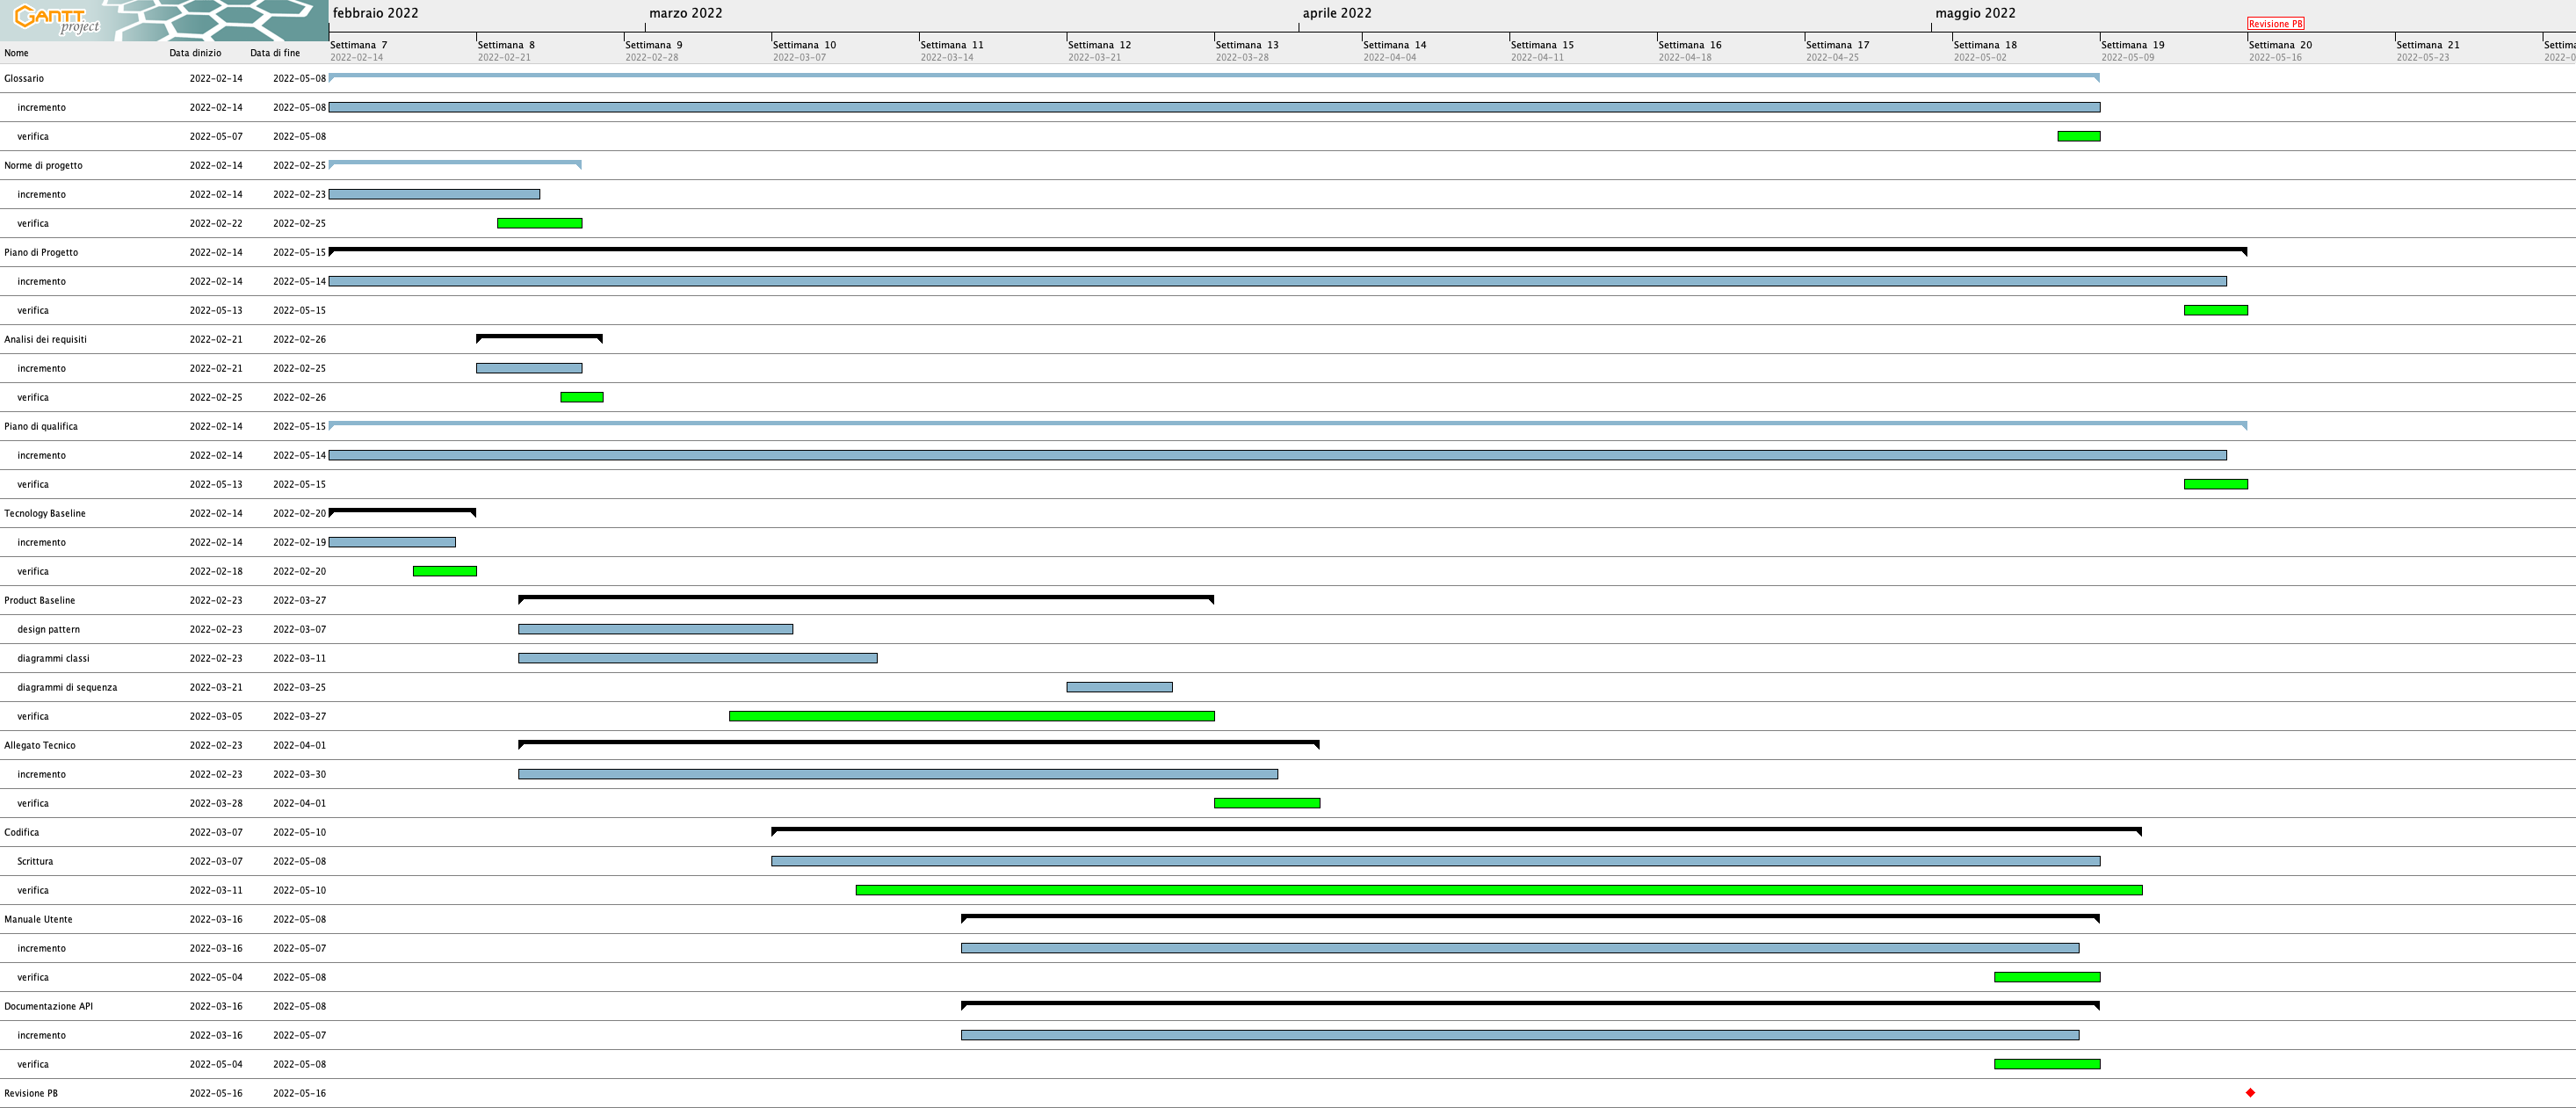
\includegraphics[width=1.5\textwidth, angle=90 ]{Sezioni/gantt/progettazione_codifica.png}
	\caption{Diagramma di Gantt - Progettazione e Codifica}
\end{figure}

